%presentation
\documentclass{beamer}

%impressions
%\documentclass[handout]{beamer}
%\usepackage{pgfpages}
%\pgfpagesuselayout{2 on 1}[a4paper,border shrink=5mm]
%\setbeameroption{notes on second screen}
%\pgfpagelayout{2 on 1}[a4paper, border, shrink=5mm]
% vue sur http://wwwtaketorg/spip/articlephp3?id_article=30...
\usepackage[T1]{fontenc}
\usepackage[frenchb]{babel}
\usepackage[utf8x]{inputenc} % Pour pouvoir taper les accents sans faire de combinaison
%\usepackage{arev}
%\usepackage{aeguill}
%mode code
\usepackage{listings}

%mode verbatim
\usepackage{moreverb}

%\usepackage[darktab]{beamerthemesidebar}
%\leftsidebar
%\usetheme{Hannover}
%\usetheme{Warsaw}
%\usetheme{PaloAlto}
\usetheme{JuanLesPins}
%\usetheme{Antibes}
%\usetheme{Shingara}
%\usetheme{Berlin}
%\usetheme{Oxygen}
\usepackage{thumbpdf}
\usepackage{wasysym}
\usepackage{ucs}
\usepackage{pgfarrows,pgfnodes,pgfautomata,pgfheaps,pgfshade}
\usepackage{verbatim}
\usepackage{color}

\title{Pictrails}
\author{Cyril Mougel}


\begin{document}

\begin{frame}
    \titlepage
\end{frame}

\begin{frame}
	\frametitle{Vous êtes un photographe ?}
    \begin{center}
    \includegraphics[scale=.3]{photographe}
    \end{center}
\end{frame}

\begin{frame}
    \frametitle{Vous faites toutes sortes de photo}
    \begin{center}
    \includegraphics[scale=.3]{belle_photo}
    \end{center}
\end{frame}

\begin{frame}
    \frametitle{Plus ou moins jolie}
    \begin{center}
    \includegraphics[scale=.1]{debile}
    \end{center}
\end{frame}

\begin{frame}
    \frametitle{Vous avez envie de les montrer au monde}
    \begin{center}
    \includegraphics[scale=.3]{world}
    \end{center}
\end{frame}

\begin{frame}
    \frametitle{Alors Pictrails est pour vous}
    \begin{center}
        \includegraphics[scale=.8]{for_you}
    \end{center}
\end{frame}

\begin{frame}
    \frametitle{Présentation}
    \begin{itemize}
        \item Galerie photo
        \item Version 0.6 (18 Novembre 2008)
        \item Rails 2.1
    \end{itemize}
\end{frame}

\section{Administration}
\begin{frame}
\tableofcontents[currentsection,currentsubsection]
\end{frame}

\begin{frame}
    \frametitle{On peux ajouter des Galeries}
    \begin{center}
    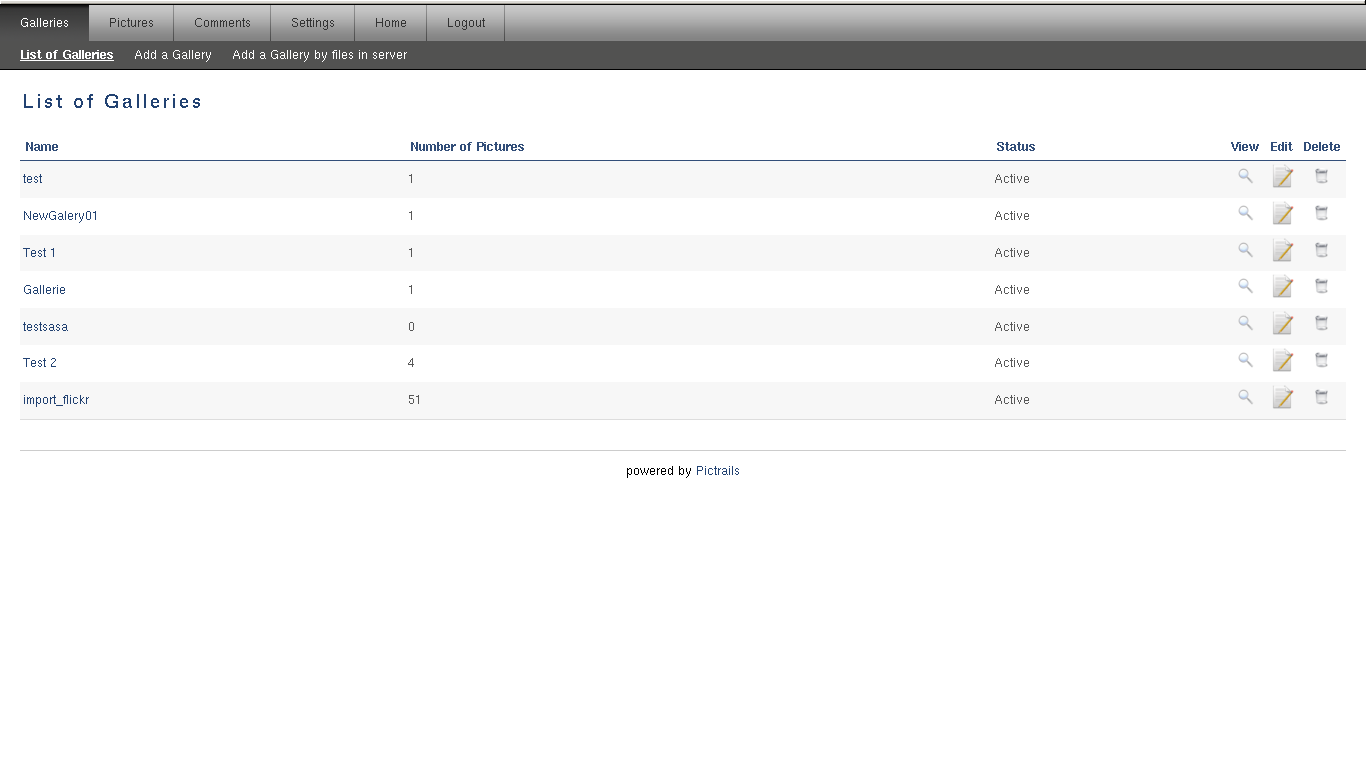
\includegraphics[scale=.4]{admin_view.png}
    \end{center}
\end{frame}

\begin{frame}
    \frametitle{On peux ajouter des photos}
    \begin{center}
    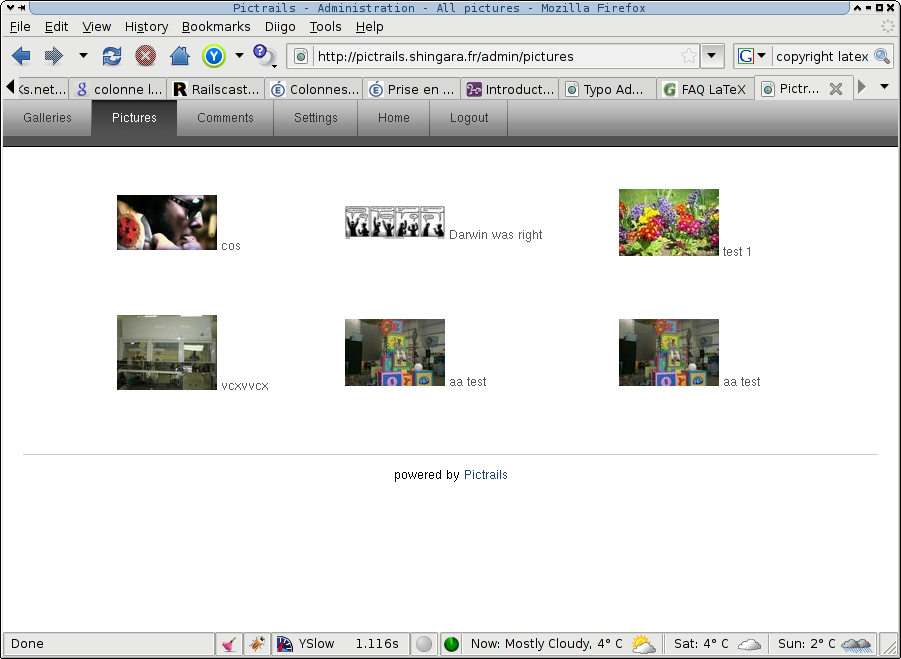
\includegraphics[scale=.4]{add_picture.png}
    \end{center}
\end{frame}

\begin{frame}
    \frametitle{On peux voir les commentaires}
    \begin{center}
    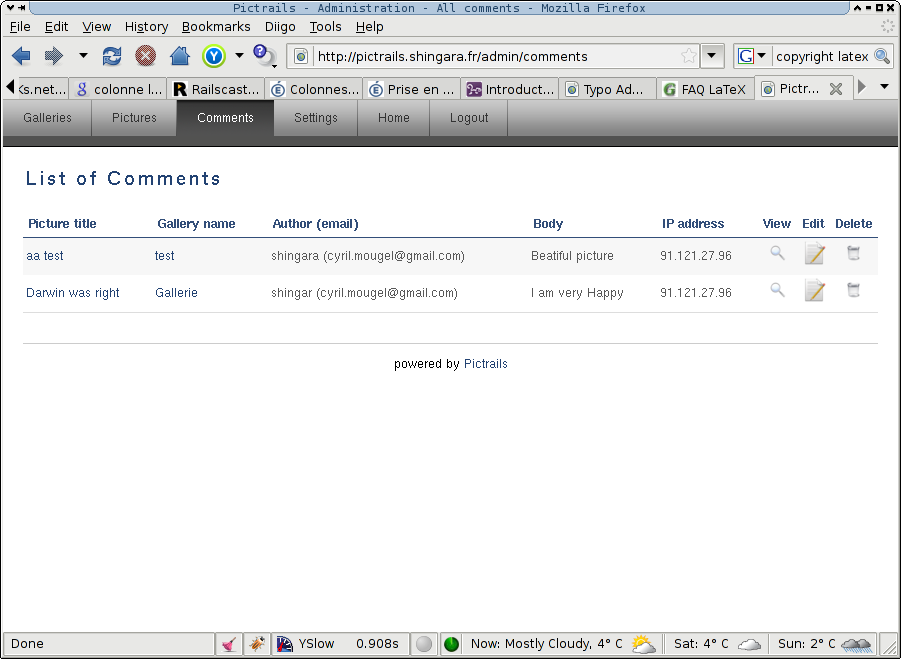
\includegraphics[scale=.4]{see_comment.png}
    \end{center}
\end{frame}

\section{Partie public}
\begin{frame}
\tableofcontents[currentsection,currentsubsection]
\end{frame}

\begin{frame}
  \frametitle{Arborescence par Galerie}
    \begin{center}
    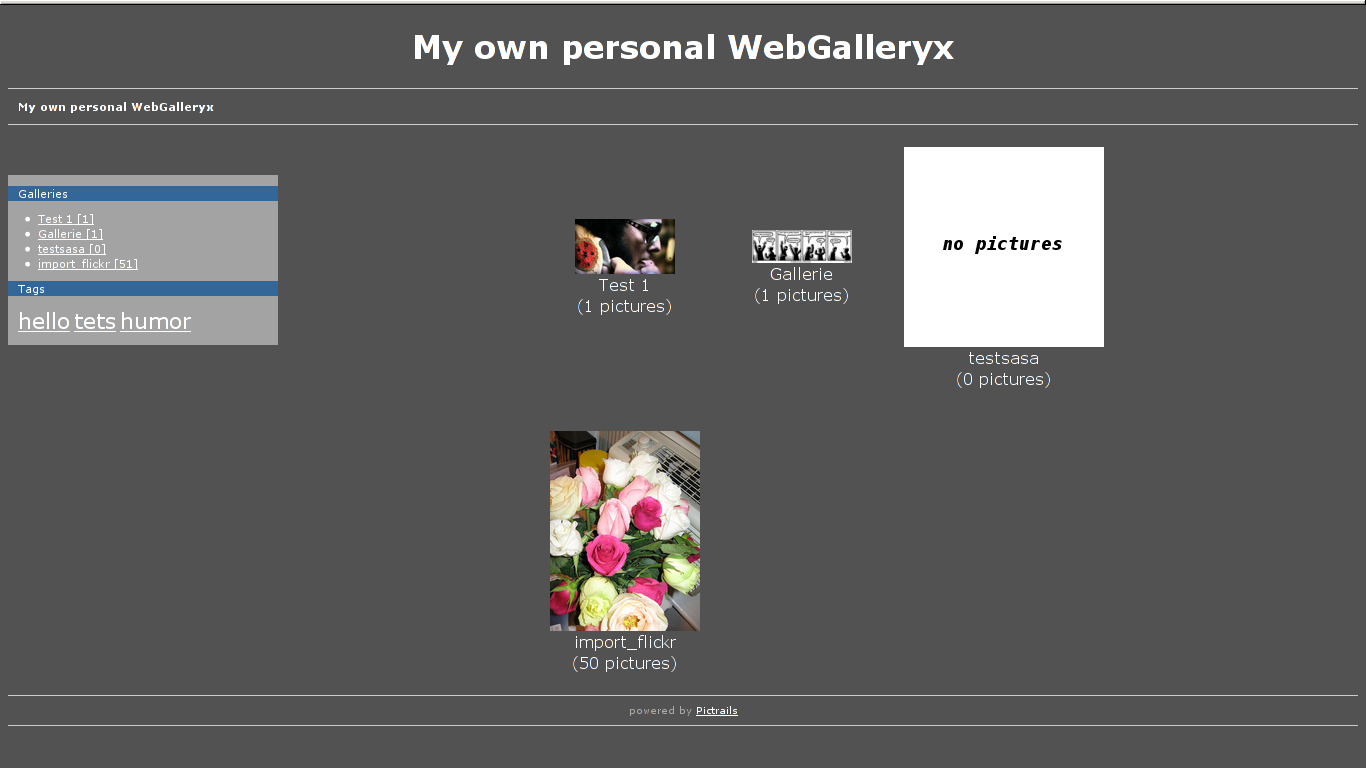
\includegraphics[scale=.4]{arborescence_gallerie.png}
    \end{center}
\end{frame}

\begin{frame}
    \frametitle{Navigation entre les photos}
    \begin{center}
    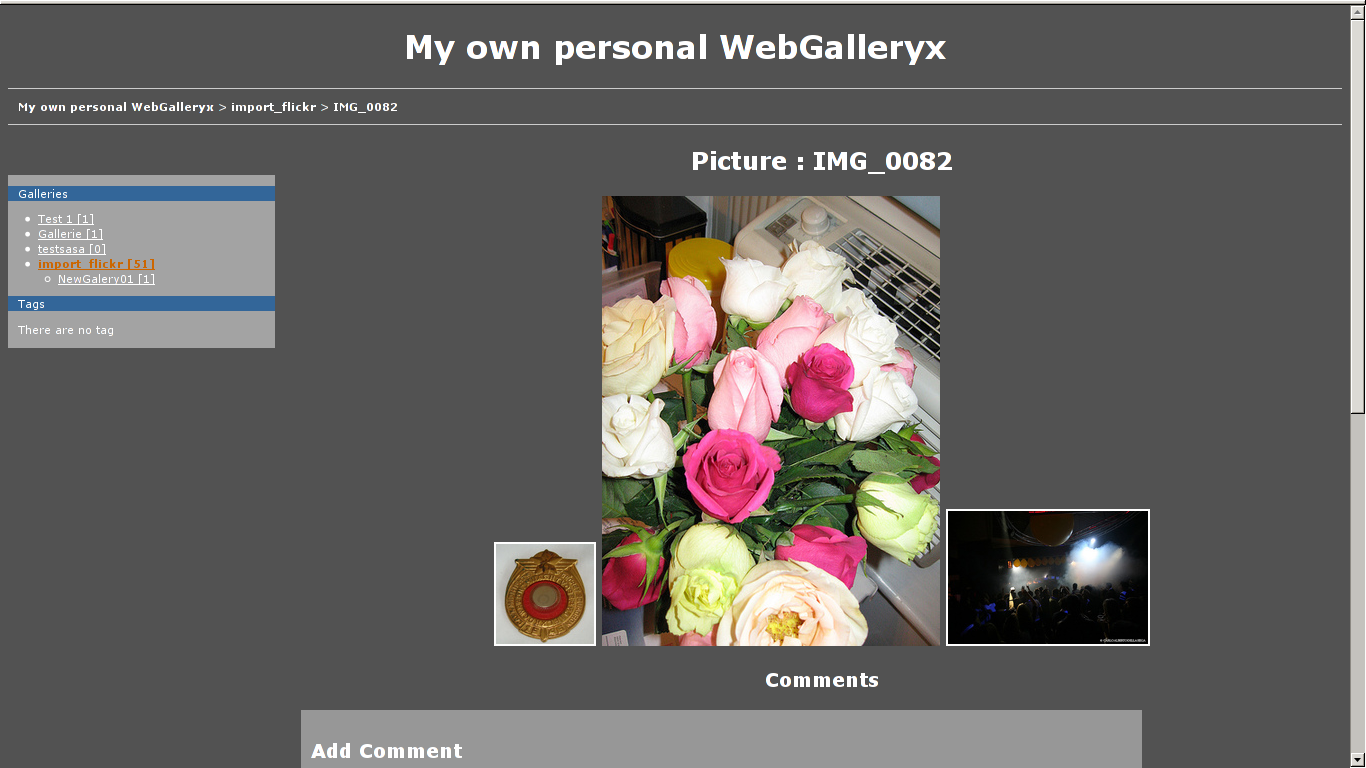
\includegraphics[scale=.3]{picture_view.png}
    \end{center}
\end{frame}

\begin{frame}
    \frametitle{Navigation par tag}
    \begin{center}
    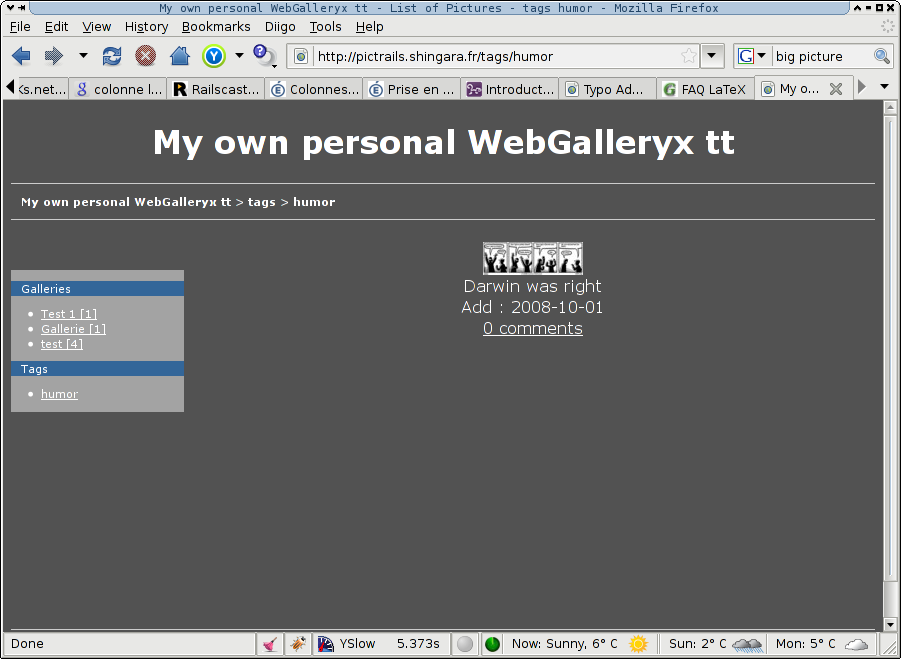
\includegraphics[scale=.4]{tag_view.png}
    \end{center}
\end{frame}

\begin{frame}
    \frametitle{Ajout de commentaires}
    \begin{center}
    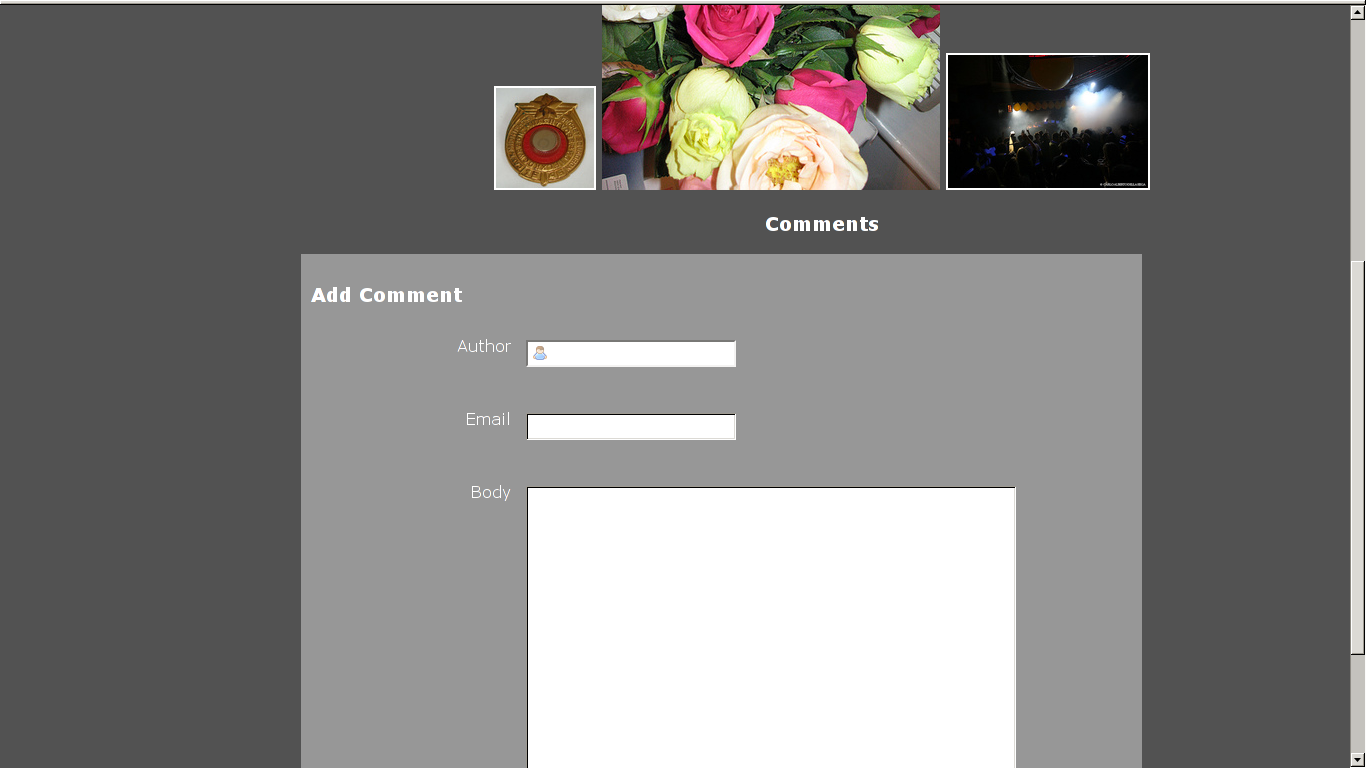
\includegraphics[scale=.3]{comment_view.png}
    \end{center}
\end{frame}

\begin{frame}
    \frametitle{La fonctionnalité qui poutre ?}
    L'ajout de galerie par Mass Upload avec progress bar sur l'avancement

    \begin{center}
    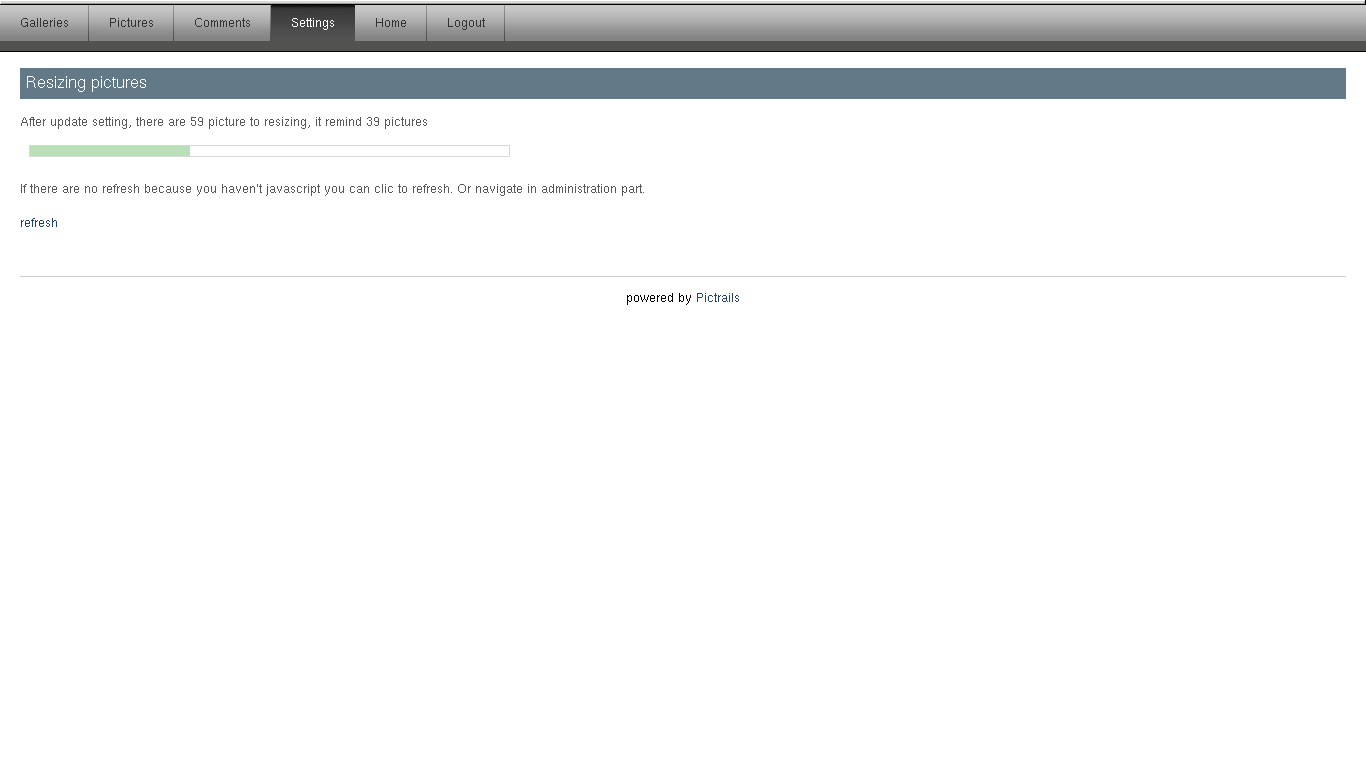
\includegraphics[scale=.4]{progress_bar.png}
    \end{center}

\end{frame}

\end{document}
